\newcommand{\anonsection}[1]{\section*{#1}\addcontentsline{toc}{section}{#1}}
\newcommand{\anonsubsection}[1]{\subsection*{#1}\addcontentsline{toc}{subsection}{#1}}
\documentclass[10pt]{article}
\usepackage{a4wide}
\usepackage[utf8]{inputenc}
\usepackage[russian]{babel}
\usepackage{graphicx}
\usepackage{amsmath}
\usepackage{amsfonts}
\usepackage{caption}
\usepackage{subfig}
\usepackage[left=3cm,right=3cm, top=3cm,bottom=3cm,bindingoffset=0cm]{geometry}
\usepackage{hyperref}

\newtheorem{theorem}{Теорема}
\newtheorem{definition}{Определение}

\begin{document}

\thispagestyle{empty}

\begin{center}
\ \vspace{-3cm}


\includegraphics[width=0.5\textwidth]{msu.png}\\
{\scshape Московский государственный университет имени М.~В.~Ломоносова}\\
Факультет вычислительной математики и кибернетики\\
Кафедра системного анализа

\vfill

{\LARGE Отчет о практическом задании по курсу ``Оптимальное управление'' }

\vspace{1cm}

{\Huge\bfseries <<Решение линейной задачи быстродействия>>}
\end{center}

\vspace{1cm}

\begin{flushright}
  \large
  \textit{Студент 315 группы}\\
  Е.\,В.~Гуров

  \vspace{5mm}

  \textit{Руководитель практикума}\\
  к.ф.-м.н., доцент П.\,А.~Точилин
\end{flushright}

\vfill

\begin{center}
Москва, 2021
\end{center}
\newpage

\tableofcontents
\newpage

\anonsection{Постановка задачи}
Задана линейная система обыкновенных дифференциальных уравнений:\\
\[ \dot{x} = Ax + Bu + f  \  , \ t \in [t_0, +\infty).\]
Здесь \(x \in \mathbb{R}^2, \ A \in \mathbb{R}^{2 \times 2}, \ B \in \mathbb{R}^{2 \times 2}, \ f \in \mathbb{R}^2, \ u \in \mathbb{R}^2 .\) На значения управляющих параметров \(u\) наложено ограничение: \(u \in \mathcal{P}.\) Пусть \( \mathcal{X}_0\) ~--- начальное множество значений фазового вектора, \(\mathcal{X}_1\) ~--- целевое множество значений фазового вектора. Необходимо решить задачу быстродействия, т.е. найти минимальное время \(T > 0\), за которое траектория системы, выпущенная в момент времени \(t_0\) из некоторой точки множества \(\mathcal{X}_0\), может попасть в некоторую точку множества \(\mathcal{X}_1\).
\bigskip
\[ \mathcal{P} = conv\{p_1, p_2, p_3, p_4\} \ , \ p_1, p_2, p_3, p_4 \in \mathbb{R}^2;\]
\[\mathcal{X}_0 = {x_0};\]
\[\mathcal{X}_1 = (\text{квадрат со стороной} \ r_1 > 0, \text{с центром в точке} \ x_1) + \] 
\[(\text{эллипсоид с матрицей конфигурации} \ Q = Q^T > 0  \ \text{и центром в нуле}).  \]

\anonsection{Теоретическая часть}

\anonsubsection{Принцип максимума Понтрягина}
Основным утверждением, которым мы будем пользоваться при поиске оптимального управления, является принцип максимума Понтрягина для линейной задачи быстродействия (см.\cite{1}). Он дает необходимые условия оптимальности для пары \( (x, u)\) ~--- управления и соответствующей ему траектории системы.\bigskip \\
Пусть дана линейная задача быстродействия:
\begin{equation}
 \begin{cases}
   \dot{x} = A(t)x + B(t)u + f(t) \ , \ t \in [t_0, t_1],
   \\
   x \in \mathbb{R}^2 \ , \ u \in \mathcal{P} \subset \mathbb{R}^2,
   \\
   x(t_0) \in \mathcal{X}_0 \ , \ x(t_1) \in \mathcal{X}_1,
   \\
   t_1 - t_0 \to \min.
 \end{cases}
 \label{problem}
\end{equation}

\noindent Рассмотрим пару
\[ (x(t), u(t)) \ , \ t_0 \leq t \leq t_1, \]
где
\begin{enumerate}
 	\item \(u(t) \in \mathcal{P}\), т.е. \( u(t) \) --- допустимое управлние, определенное на отрезке \( t_0 \leq t \leq t_1 \), причем в каждый момент времени \(t \in [t_0, t_1] \) значение \( u(t) \in \mathcal{P} \).
 	\item \( x(t) \) --- траектория, отвечающая управлению \( u(t) \), т.е. \( \dot{x}(t) = Ax(t) + Bu(t) + f(t) \) для почти всех \( t \in [t_0, t_1] \), и удовлетворяющая краевым условиям \( x(t_0) \in \mathcal{X}_0, \ x(t_1) \in \mathcal{X}_1 \).
\end{enumerate}
Будем говорить , что эта пара \( (x(t), u(t)) \) \emph{удовлетворяет принципу максимума Понтрягина на отрезке} \( [t_0, t_1] \), если существует такая \( \psi(t) \in \mathbb{R}^2\) ~--- сопряженная переменная, являющаяся решением сопряженной задачи:
\[ \dot{\psi}(t) = -A^T(t) \psi(t) \ , \ \psi(t) \neq 0,\]
что выполнены следующие три условия:
\begin{enumerate}
	\item Условие максимума: \( \langle \psi(t), B(t)u(t) \rangle = \rho(B(t) \mathcal{P}(t) , \psi(t))\) для почти всех \( t \in [t_0, t_1]. \)
	\item Условие трансверсальности на левом конце: \( \langle \psi(t_0), x(t_0) \rangle = \rho(\mathcal{X}_0 , \psi(t_0)).\)
	\item Условие трансверсальности на правом конце: \(\langle -\psi(t_1), x(t_1) \rangle = \rho(\mathcal{X}_1 , -\psi(t_1)).\)
\end{enumerate}

\begin{theorem}[Основная теорема линейной теории быстродействия]
	Пусть
	\begin{enumerate}
		\item \( \mathcal{X}_0, \mathcal{X}_1 \in conv \Omega( \mathbb{E}^{n}),\)
		\item Пара \( (x(t), u(t)) \ , \ t_0 \leq t \leq t_1\), решает линейную задачу быстродействия (\ref{problem}), т.е 
		 \[ u(t) \in \mathcal{P}, \ x(t_0) \in \mathcal{X}_0, \ x(t_1) \in \mathcal{X}_1, \ t_1 - t_0 = \min. \]
	\end{enumerate}
	Тогда пара \( (x(t), u(t)) \) удовлетворяет принципу максимума Понтрягина на отрезке \( [t_0, t_1] \).
\end{theorem}

\anonsubsection{Вычисление опорных функций для множества начальных состояний, целевого множества и множества допустимых управлений}
Перечислим свойства, необходимые для вычисления требуемых опорных функций\medskip\\
\textbf{Свойство} \(1^{\circ}\) (\textit{положительная однородность по первому аргументу}):
\[ \rho( \alpha X, \psi) = \alpha \cdot \rho(X, \psi) \ , \ \forall \alpha \geq 0 \ , \ \psi \in \mathbb{E}^n.\]
\textbf{Свойство} \(2^{\circ}\) (\textit{аддитивность по первому аргументу}):
\[ \rho(X_1 + X_2, \psi) = \rho(X_1, \psi) + \rho(X_2, \psi).\]
\textbf{Свойство} \(3^{\circ}\) (\textit{опорная функция линейно преобразованного множества}):\\
пусть \(D\) - квадратная матрица \(n\)-го порядка, тогда
\[ \rho(DX, \psi) = \rho(X, D^T\psi) \ , \ \forall \psi \in \mathbb{E}^n.\]
\textbf{Свойство} \(4^{\circ}\) (\textit{совпадение опорных функций множества и его наименьшей выпуклой оболочки}):
\[ \rho(X,\psi) = \rho(conv (X), \psi) \ , \ \forall \psi \in \mathbb{E}^n. \bigskip \]
Перейдем теперь к подсчету функций множеств, фигурирующих в Принципе максимума.\medskip\\
\textbf{Множество} \( \mathcal{X}_0\):\smallskip\\
Опорная функция множества начальных состояний, состоящего из единственной точки \(x_0\) находится очевидно.
\[ \rho(\mathcal{X}_0, \psi) = \langle x_0, \psi \rangle \ , \ \forall \psi \in \mathbb{E}^2.\] 
\textbf{Множество} \( \mathcal{P}\):\smallskip\\
Пользуясь свойством 4, немедленно получаем опорную функцию множества допустимых управлений.
\[ \rho(\mathcal{P}, \psi) = \rho(conv(\{p_1, p_2, p_3, p_4\}), \psi) = \rho(\{p_1, p_2, p_3, p_4\}, \psi) = \max\limits_{i} \langle p_i, \psi \rangle \ ,\ i = \overline{1, 4} \ , \ \forall \psi \in \mathbb{E}^2.\] 
В формулировке Принципа максимума Понтрягина фигурирует опорная функция множества \(B \mathcal{P} \). Для перехода к опорной функции такого множества воспользуемся свойством 3 и получим:
\[ \rho(B \mathcal{P}, \psi) = \rho(\mathcal{P}, B^T \psi) = \max\limits_{i} \langle p_i, B^T \psi \rangle \ , \ i = \overline{1,4} \ , \ \forall \psi \in \mathbb{E}^2.\]
\textbf{Множество} \( \mathcal{X}_1\):\smallskip\\
Пользуясь свойствами 1, 2, 3 найдем опорную функцию целевого множества.\medskip\\
1)Опорная функция квадрата: 
\[ \rho (X_{r_1},\psi) = \rho(r_1 X_1, \psi) = r_1 \cdot \rho(X_1, \psi) = r_1 \cdot  \smash{\displaystyle\max_{x \in X_1}} ( x, \psi) = r_1 \cdot \smash{\displaystyle\max_{|x_1| \leq 1, |x_2| \leq 1}}(x_1 \psi_1 + x_2 \psi_2) =  r_1(|\psi_1| + |\psi_2|). \bigskip\]
2)Опорная функция эллипса с заданной матрицей конфигурации \(Q = Q^T > 0\) и центром в нуле:
\[ \rho(E_Q, \psi) = \rho(Q * B_1, \psi) = \rho(B_1, Q^T \psi) = \rho(B_1, Q\psi) = \|Q\psi\| \ , \ \forall \psi \in \mathbb{E}^2.\]
Здесь \( B_1 \) ~--- это шар радиуса 1 с центром в точке 0. Опорная функция такого множества представляется в виде:
\[ \rho(B_1, \psi) = \max\limits_{x \in B} \langle x, \psi \rangle  =  \langle \frac{\psi}{ \| \psi \| }, \psi \rangle  = \| \psi \| \ , \ \forall \psi \in \mathbb{E}^2.\]
3)Множество \( \mathcal{X}_1\) представляет собой сумму трех множеств: точки \( x_1\), квадрата со стороной \(r_1\) и центром в нуле и эллипса с матрицей конфигурации \( Q = Q^T > 0\) и центром в нуле. Его опорная функция представляется в виде:
\[ \rho(\mathcal{X}_1, \psi) = \rho(x_1, \psi) + \rho(X_{r_1}, \psi) + \rho(E_Q, \psi) =  \langle x_1, \psi \rangle + \, r_1 (|\psi_1| + |\psi_2|) + \|Q\psi\| \ , \ \forall \psi \in \mathbb{E}^2.\]

\anonsubsection{Описание алгоритма работы программы}
Алгоритм поиска оптимальных управлений основывается на переборе различных \( u \in \mathcal{P} \), удовлетворяющих Принципу максимума Понтрягина, то есть потенциально оптимальных. Таким образом ПМП позволяет значительно сузить границы рассматриваемых управлений и уменьшить вычислительную сложность задачи. При этом из принципа максимума следует, что каждой сопряженной переменной соответсвует некоторое управление \( u^* \), потенциально оптимальное. Поэтому, перебирая начальные условия в сопрженной задаче, мы автоматически будем перебирать управления \( u* \), и решив для каждого из них систему ОДУ из условия задачи, сможем выбрать оптимальное в смысле времени.\bigskip\\
\textbf{1.} Перебираем начальные условия \( \psi(t_0) \) в сопряженной задаче. Для систематизации перебора имеет смысл нормировать начальные условия и выбирать их на единичной окружности, так как \( \underset{u(\cdot) \in \mathcal{P}}{\text{Argmax}} \langle u(t), B^T \psi(t) \rangle = \underset{u(\cdot) \in \mathcal{P}}{\text{Argmax}} \langle u(t), B^T (\alpha \psi(t)) \rangle \ , \ \forall \alpha > 0. \)\medskip\\
\textbf{2.} Для выбранного начального условия \( \psi(t_0) \) найдем \( \psi(t) \) - решение сопряженной задачи. В силу стационарности системы \( \psi(t) = e^{-(t - t_0)A^{T}}\psi(t_0) \).\medskip\\
\textbf{3.} С помощью опорной функции множества допустимых управлений по полученной \( \psi(t) \) из условия максимума найдем \( u^*(t) \) как опорный вектор.\medskip\\
\textbf{4.} Для найденного \( u^*(t) \) с помощью функции ode45 решим сисстему ОДУ из условия задачи. Окончанием процесса интегрирования будет достижение максимального наперед заданного \( T_{max} \) или целевого множества.\medskip\\
\textbf{5.} Для траекторий, достигших целевого множества, выберем решение с наименьшим временем.

\anonsubsection{Комментарий к численному методу}
Важно отметить особенность реализации проверки условия попадания фазовой траектории в целевое множество. В основе нее лежит тот факт, что функция, сопряженная к опорной функции выпуклого множества ~--- это характеристическая функция этого множества (см.\cite{2}). Она принимает значение 0 внутри множества и \( + \infty \) вне его. 

\begin{definition}
	Пусть задана функция \( f: X \to \overline{\mathbb{R}} \) . Преобразованием Юнга-Фенхеля функции \( f \), или функцией сопряженной к \( f \), называется функция, определенная формулой: 
	\[ f^{*}(x^{*})=\sup _{x\in X} ( \langle x^{*} , x \rangle -f(x) ). \]
\end{definition}

Отметим, что если \( X \) ~--- линейное нормированное пространство, то сопряженная функция \( f^{*} \) определяется на сопряженном пространстве \( X^{*} \) линейных непрерывных функционалов \( x^{*} \) на \( X \). В данном случае \( \mathbb{R}^2 \) ~--- гильбертово пространство, и \( X \) изоморфно \( X^{*} \) .\smallskip\\
В программной реализации супремум из определения сопряженной функции ищется с помощью matlab-функции `` fminunc '', которая минимизирует функцию-аргумент безусловно, то есть на всем пространстве. Для уточнения её работы, квадрат, являющийся слагаемым в целевом множестве, апроксимируется шаром по норме \( p \). При достаточно больших \( p \) апроксимация является довольно точной.\smallskip\\
Опорная функция единичного шара по норме \( p \) является сопряженной нормой к \(p\)-норме, то есть \(q\)-нормой, где \(q \) ищется из соотнощения:
\[ \frac{1}{p} + \frac{1}{q} = 1. \]
Тогда опорная функция целевого множества примет вид:
\[ \rho(\mathcal{X}_1, \psi) =  \langle x_1, \psi \rangle + \, r_1 \cdot \|\psi\|_q + \|Q\psi\| \ , \ \forall \psi \in \mathbb{E}^2.\]

\anonsubsection{Погрешность условия трансверсальности}
Так как внутри алгоритма условие трансверсальности на правом конце при отборе оптимальных пар не проверяется, оно может не выполняться в точности. Поэтому отметим погрешность этого условия, которую будем считать как аболютное значение разности:
\[ \langle -\psi(t_1), x^*(t_1) \rangle - \rho(\mathcal{X}_1 , -\psi(t_1)). \]
Здесь \( \psi(t_1) \) ~--- вектор сопряженной переменной в момент попадания фазовой траектории в целевое множество.

\anonsubsection{Параметры численного метода}
Перечислим параметры программы, которые можно изменять для уточнения конечного результата. 
\begin{itemize}
	\item absTol, relTol ~--- абсолютная и относительная ошибки для решателя ode45.
	\item pNorm ~--- норма, по которой квадрат, являющийся слагаемым в целевом множестве, апроксимируется шаром.
	\item number of iterations ~--- количество фазовых траекторий, которые будут выпущены из множества \( \mathcal{X}_0 \). 
	\item maximum integration time ~--- максимальное время интегрирования для каждой траектории. Если множество не достигнуто имеет смысл увеличить время интегрирования.
\end{itemize}
\newpage
\anonsection{Примеры работы программы для разных параметров задачи.}
\anonsubsection{Пример 1}
\[ A = \begin{bmatrix}
      		1 & -1 \\[0.3em]
      		1 & 1
      	  \end{bmatrix} , 
 B = \begin{bmatrix}
      	   3 & 0 \\[0.3em]
      	   0 & 3
      \end{bmatrix} ,
 f = \begin{bmatrix}
       	    0 \\[0.3em]
      	    0
      \end{bmatrix} ,
 x_0 = \begin{bmatrix}
      	    1 \\[0.3em]
      	    1
      \end{bmatrix} ,
 x_1 = \begin{bmatrix}
      	7 \\[0.3em]
      	10
      \end{bmatrix} ,
 Q = \begin{bmatrix}
      	   1 & -1 \\[0.3em]
      	   -1 & 2
      \end{bmatrix}, \]
\[ p_1 = \begin{bmatrix}
      	-1 \\[0.3em]
      	-1
      \end{bmatrix} ,
p_2 = \begin{bmatrix}
      	-1 \\[0.3em]
      	1
      \end{bmatrix} ,
p_3 = \begin{bmatrix}
      	1 \\[0.3em]
      	1
      \end{bmatrix} ,
p_4 = \begin{bmatrix}
      	1 \\[0.3em]
      	-1
      \end{bmatrix}, r_1 = 3 \]
\[ t_0 = 0, \text{absTol = 1e-7, relTol = 1e-6, pNorm = 10, number of iterations = 100}\]  
\[\text{maximum integration time = 2} \]
\textbf{Результат:} Оптимальное время:1.159331; ошибка условия трансверсальности на правом конце:0.000059 

\begin{figure}[h]
    \centering
    \subfloat[\centering Траектории системы в фазовом пространстве.]{{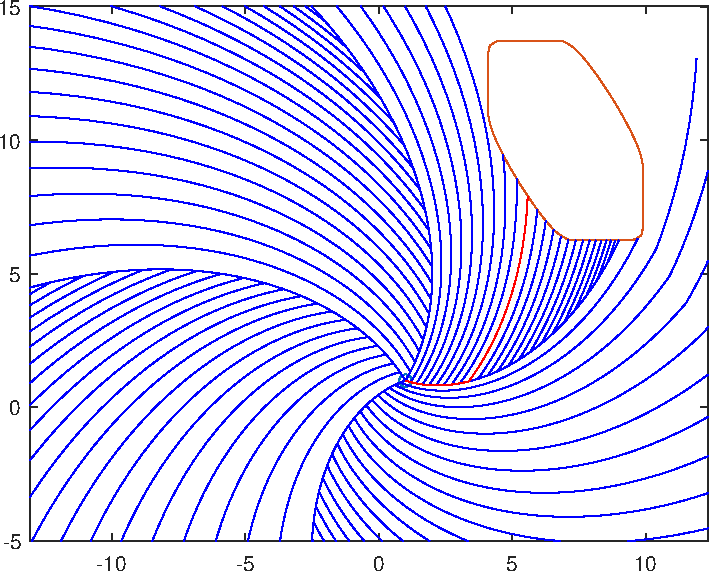
\includegraphics[width=7cm]{Phase_space_1.pdf} }}
    \qquad
    \subfloat[\centering Графики компонент оптимального управления \( u(t) \).]{{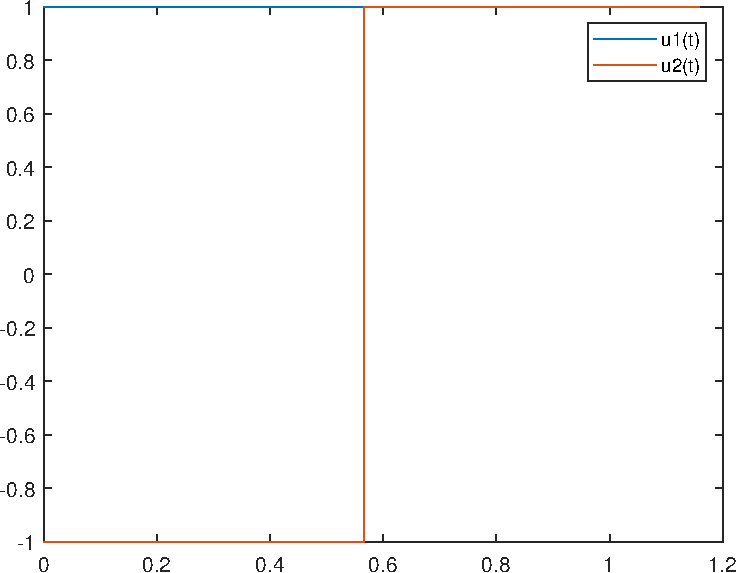
\includegraphics[width=7cm]{u(t)_1.pdf} }}
    \\
    \subfloat[\centering Графики компонент оптимальной траектории \( x(t) \).]{{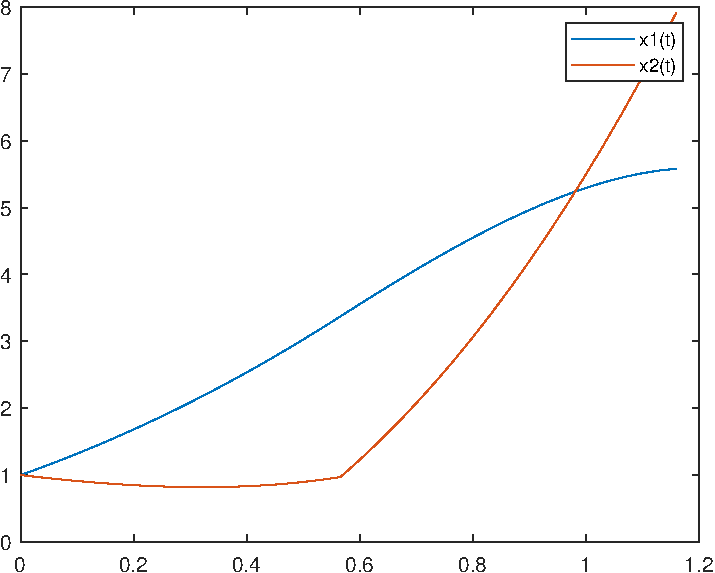
\includegraphics[width=7cm]{x(t)_1.pdf} }}
    \qquad
    \subfloat[\centering Графики компонент сопряженной переменной \( \psi(t) \).]{{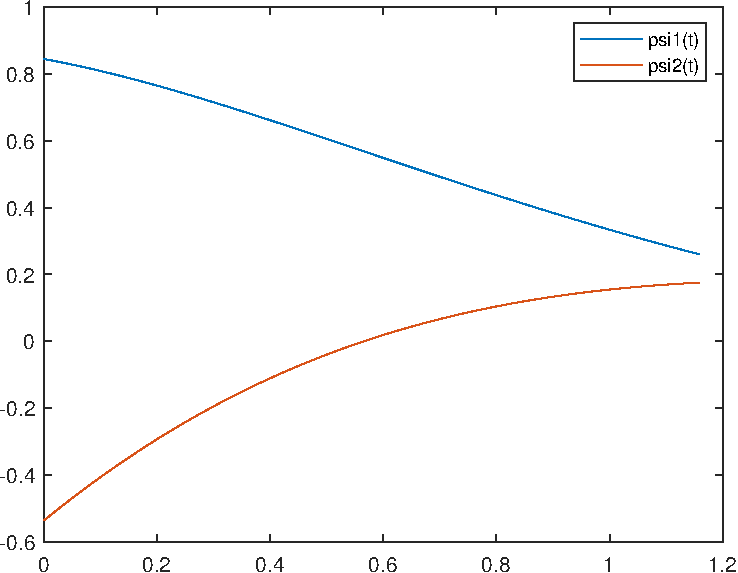
\includegraphics[width=7cm]{psi(t)_1.pdf} }}
\end{figure}

\newpage
\anonsubsection{Пример 2}
 \[ A = \begin{bmatrix}
      		0 & -2 \\[0.3em]
      		3 & 0
      	  \end{bmatrix} , 
 B = \begin{bmatrix}
      	   1 & -1 \\[0.3em]
      	   2 & 3
      \end{bmatrix} ,
 f = \begin{bmatrix}
       	    1 \\[0.3em]
      	    2
      \end{bmatrix} ,
 x_0 = \begin{bmatrix}
      	    2 \\[0.3em]
      	    3
      \end{bmatrix} ,
 x_1 = \begin{bmatrix}
      	9 \\[0.3em]
      	7
      \end{bmatrix} ,
 Q = \begin{bmatrix}
      	   1 & 1 \\[0.3em]
      	   1 & 2
      \end{bmatrix}, \]
\[ p_1 = \begin{bmatrix}
      	-1 \\[0.3em]
      	-1
      \end{bmatrix} ,
p_2 = \begin{bmatrix}
      	-1 \\[0.3em]
      	1
      \end{bmatrix} ,
p_3 = \begin{bmatrix}
      	1 \\[0.3em]
      	1
      \end{bmatrix} ,
p_4 = \begin{bmatrix}
      	1 \\[0.3em]
      	-1
      \end{bmatrix}, r_1 = 3 \]
\[ t_0 = 0, \text{absTol = 1e-7, relTol = 1e-7, pNorm = 10, number of iterations = 60}\]  
\[\text{maximum integration time = 4} \]
\textbf{Результат:} Оптимальное время:2.127695 ; ошибка условия трансверсальности на правом конце:0.362278 

\begin{figure}[h]
    \centering
    \subfloat[\centering Траектории системы в фазовом пространстве.]{{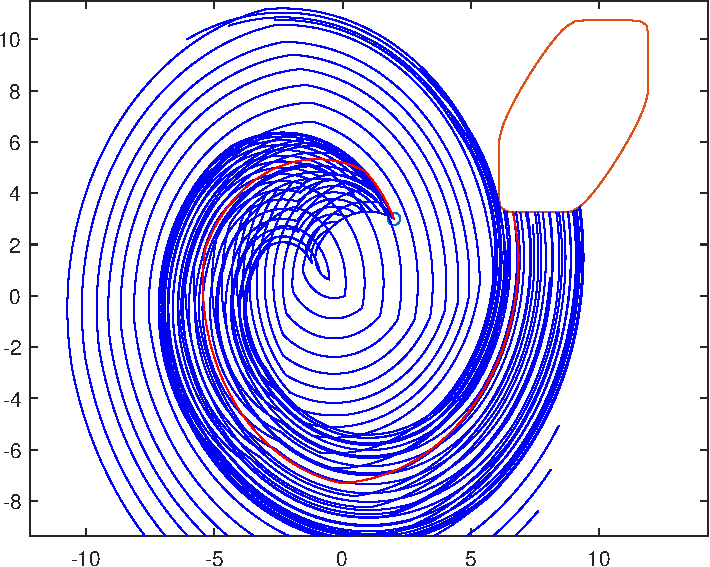
\includegraphics[width=7cm]{Phase_space_2.pdf} }}
    \qquad
    \subfloat[\centering Графики компонент оптимального управления \( u(t) \).]{{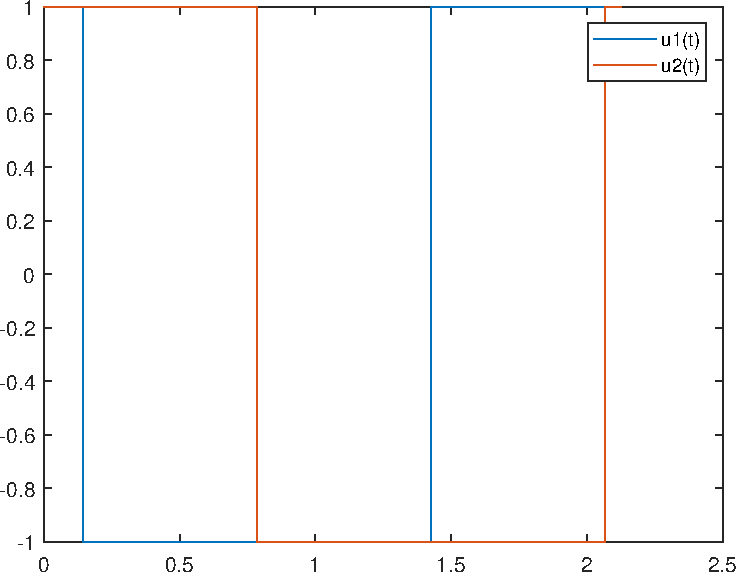
\includegraphics[width=7cm]{u(t)_2.pdf} }}
    \\
    \subfloat[\centering Графики компонент оптимальной траектории \( x(t) \).]{{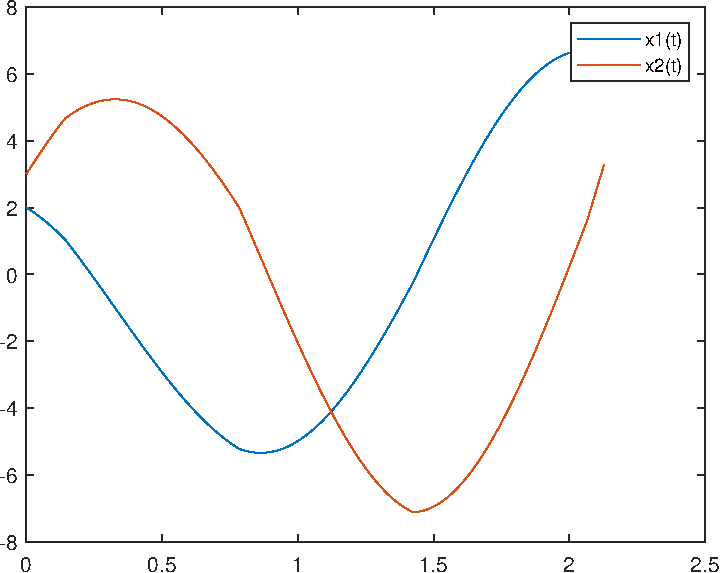
\includegraphics[width=7cm]{x(t)_2.pdf} }}
    \qquad
    \subfloat[\centering Графики компонент сопряженной переменной \( \psi(t) \).]{{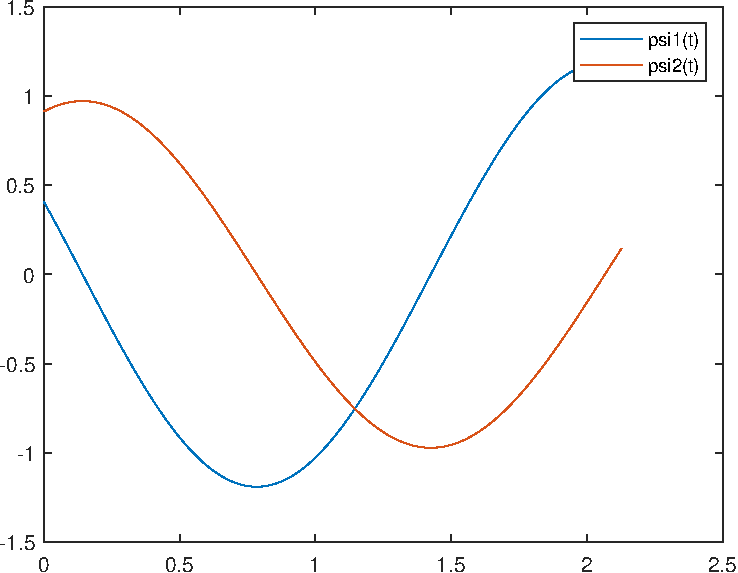
\includegraphics[width=7cm]{psi(t)_2.pdf} }}
\end{figure}

\anonsubsection{Пример 3. Иллюстрация разрывности времени оптимального быстродействия}
Данный пример иллюстрирует разрывность времени оптимального быстродействия относительно целевого множества. 
 \[ A = \begin{bmatrix}
      		1 & -5 \\[0.3em]
      		1 & -1
      	  \end{bmatrix} , 
 B = \begin{bmatrix}
      	   0.5 & 0 \\[0.3em]
      	   0 & 0.2
      \end{bmatrix} ,
 f = \begin{bmatrix}
       	    1 \\[0.3em]
      	    2
      \end{bmatrix} ,
 x_0 = \begin{bmatrix}
      	    2 \\[0.3em]
      	    3
      \end{bmatrix} ,
 x_1(a) = \begin{bmatrix}
      	-4 \\[0.3em]
      	-3.4
      \end{bmatrix} ,
x_1(b) = \begin{bmatrix}
      	-4 \\[0.3em]
      	-3.5
      \end{bmatrix} ,
 Q = \begin{bmatrix}
      	   1 & -1 \\[0.3em]
      	   -1 & 2
      \end{bmatrix}, \]
\[ p_1 = \begin{bmatrix}
      	-1 \\[0.3em]
      	-1
      \end{bmatrix} ,
p_2 = \begin{bmatrix}
      	-1 \\[0.3em]
      	1
      \end{bmatrix} ,
p_3 = \begin{bmatrix}
      	1 \\[0.3em]
      	1
      \end{bmatrix} ,
p_4 = \begin{bmatrix}
      	1 \\[0.3em]
      	-1
      \end{bmatrix}, r_1 = 4 \]
\[ t_0 = 0, \text{absTol = 1e-7, relTol = 1e-6, pNorm = 10, number of iterations = 8}\]  
\[\text{maximum integration time = 3} \]
\textbf{Результат(a):} Оптимальное время:0.683896; ошибка условия трансверсальности на правом конце:0.006446 \\
\textbf{Результат(b):} Оптимальное время:1.388466; ошибка условия трансверсальности на правом конце:0.298559 

\begin{figure}[h]
    \centering
    \subfloat[\centering Траектории системы при \( x_1(2) = -3.4 \)]{{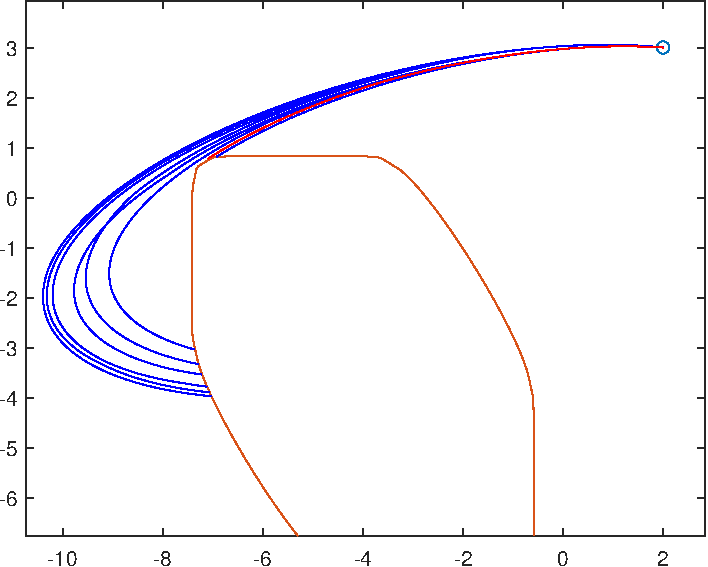
\includegraphics[width=7cm]{Phase_space_3.pdf} }}
    \qquad
    \subfloat[\centering  Траектории системы при \( x_1(2) = -3.5 \)]{{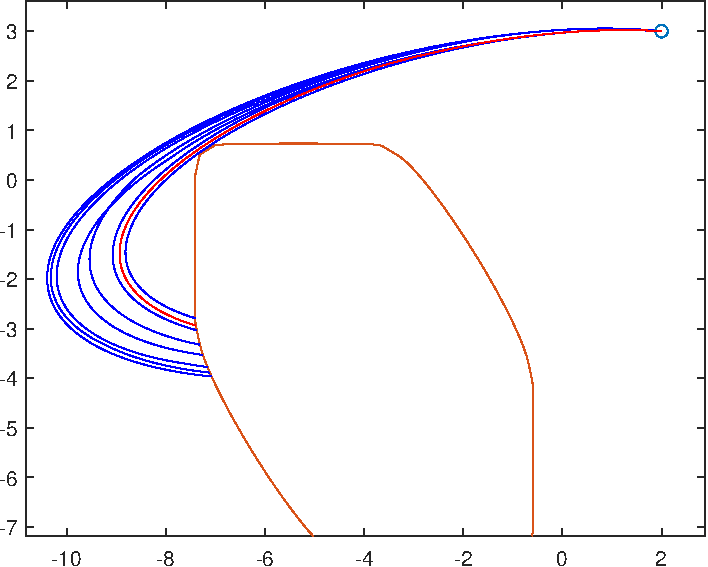
\includegraphics[width=7cm]{Phase_space_4.pdf} }}
\end{figure}

Из примера видно, что при незначительном изменении целевого множества, время оптимального быстродействия может значительно меняться.
\newpage

\anonsubsection{Пример 4. Демонстрация улучшения результата, посредством изменения параметров численного метода}
Главным параметром, влияющим на точность результата является количество итераций, или иначе, траекторий, выпущенных из множества начальных состояний. Рассмотрим снова систему из Примера 1 с двумя разными значениями number of iterations.
\[ A = \begin{bmatrix}
      		1 & -1 \\[0.3em]
      		1 & 1
      	  \end{bmatrix} , 
 B = \begin{bmatrix}
      	   3 & 0 \\[0.3em]
      	   0 & 3
      \end{bmatrix} ,
 f = \begin{bmatrix}
       	    0 \\[0.3em]
      	    0
      \end{bmatrix} ,
 x_0 = \begin{bmatrix}
      	    1 \\[0.3em]
      	    1
      \end{bmatrix} ,
 x_1 = \begin{bmatrix}
      	7 \\[0.3em]
      	10
      \end{bmatrix} ,
 Q = \begin{bmatrix}
      	   1 & -1 \\[0.3em]
      	   -1 & 2
      \end{bmatrix}, \]
\[ p_1 = \begin{bmatrix}
      	-1 \\[0.3em]
      	-1
      \end{bmatrix} ,
p_2 = \begin{bmatrix}
      	-1 \\[0.3em]
      	1
      \end{bmatrix} ,
p_3 = \begin{bmatrix}
      	1 \\[0.3em]
      	1
      \end{bmatrix} ,
p_4 = \begin{bmatrix}
      	1 \\[0.3em]
      	-1
      \end{bmatrix}, r_1 = 3 \]
\[ t_0 = 0, \text{absTol = 1e-7, relTol = 1e-6, pNorm = 10, number of iterations(a) = 20} \]  
\[\text{ number of iterations(b) = 100, maximum integration time = 2} \]
\textbf{Результат(a):} Оптимальное время:1.197213; ошибка условия трансверсальности на правом конце:0.235911 \\
\textbf{Результат(b):} Оптимальное время:1.159331; ошибка условия трансверсальности на правом конце:0.000059

\begin{figure}[h]
    \centering
    \subfloat[\centering Выпущено 20 траекторий]{{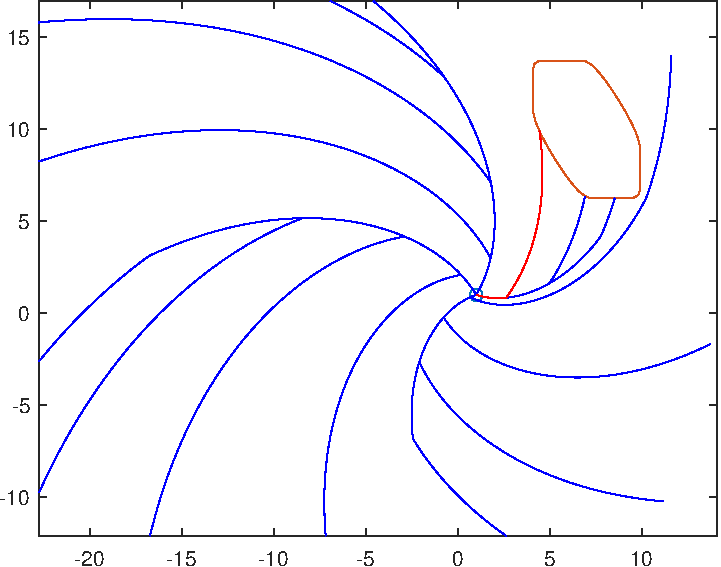
\includegraphics[width=7cm]{Phase_space_5.pdf} }}
    \qquad
    \subfloat[\centering  Выпущено 100 траекторий]{{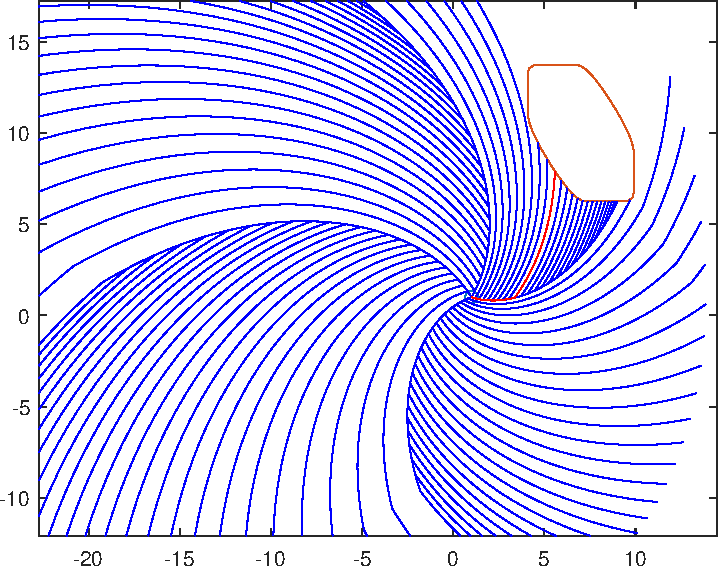
\includegraphics[width=7cm]{Phase_space_6.pdf} }}
\end{figure}

Из примера видно, что при увеличении итераций оптимальное время быстродействия улучшилось, и ошибка условия трансверсальности на правом конце сократилась на несколько порядков.
\newpage

\begin{thebibliography}{0}
\addcontentsline{toc}{section}{Список литературы}
\bibitem{1}
Ю.\,Н. Киселев, С.\,Н. Аввакумов, М.\,В. Орлов \emph{Оптимальное управление. Линейная теория и приложения:Учебное пособие} М.:МАКС Пресс, 2007
\bibitem{2}
А.\,В. Арутюнов \emph{Лекции по выпуклому и многозначному анализу} М.: Физматлит, 2014
\end{thebibliography}
\end{document}